
%%% Local Variables: 
%%% mode: latex
%%% TeX-master: t
%%% End: 

\section{Introduction}

The virtual object layer is an abstraction layer in the HDF5 library that intercepts all API calls that could potentially access objects in an HDF5 container and forwards those calls to a VOL connector, which implements the storage. The user or application gets the benefit of using the familiar and widely-used HDF5 data model and API, but can map the physical storage of the HDF5 file and objects to storage that better meets the application's data needs.

\subsection{The VOL Abstraction Layer}

The VOL lies just under the public API. When a storage-oriented public API call is made, the library performs a few sanity checks on the input parameters and then immediately invokes a VOL callback, which resolves to an implementation in the VOL connector that was selected when opening or creating the file. The VOL connector then performs whatever operations are needed before control returns to the library, where any final library operations such as assigning IDs for newly created/opened datasets are performed before returning. This means that, for calls that utilize the VOL, all of the functionality is deferred to the VOL connector and the HDF5 library does very little work. An important consideration of this is that most of the HDF5 caching layers (metadata and chunk caches, page buffering, etc.) will not be available as those are implemented in the HDF5 native VOL connector and cannot be easily reused by external connectors.

\begin{figure}[h]
\caption {The VOL Architecture}
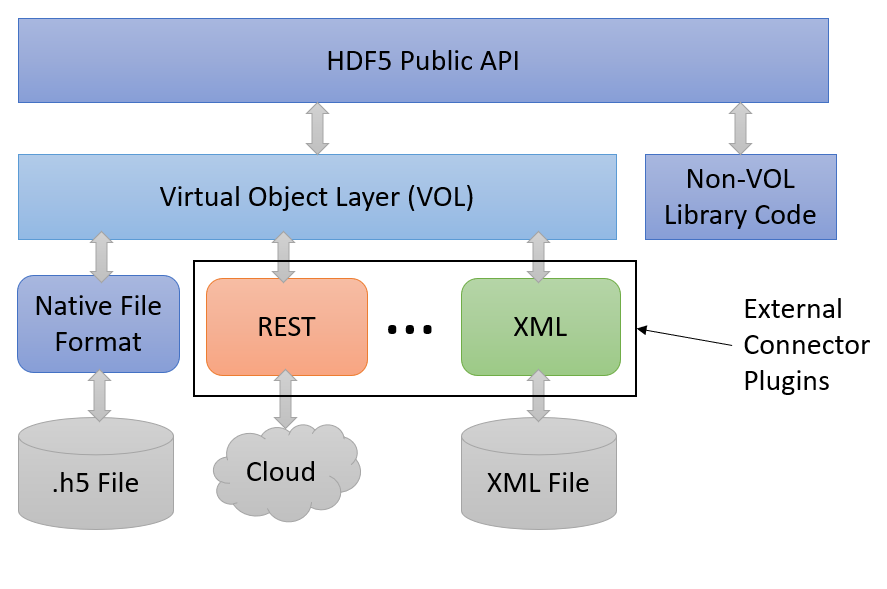
\includegraphics[width=\textwidth]{vol_architecture.png}
\end{figure}

Not all public HDF5 API calls pass through the VOL. Only calls which require manipulating storage go through the VOL and require a VOL connector author to implement the appropriate callback. Dataspace, property list, error stack, etc. calls have nothing to do with storage manipulation or querying and do not use the VOL. This may be confusing when it comes to property list calls, since many of those calls set properties for storage. Property lists are just collections of key-value pairs, though, so a particular VOL connector is not required to set or get properties.

Another thing to keep in mind is that not every VOL connector will implement the full HDF5 public API. In some cases, a particular feature like variable-length types may not have been developed yet or may not have an equivalent in the target storage system. Also, many HDF5 public API calls are specific to the native HDF5 file format and are unlikely to have any use in other VOL connectors. A feature/capabilities flag scheme is being developed to help navigate this.

For more information about which calls go through the VOL and the mechanism by which this is implemented, see the connector author and library internals documentation.

\subsection{VOL Connectors}

A VOL connector can be implemented in several ways: as a shared or static library linked to an application; as a dynamically loaded plugin, implemented as a shared library; and even as an internal connector, built into the HDF5 library itself. This document mostly focuses on external connectors, both libraries and plugins, as those are expected to be much more common than internal implementations.

Many VOL connectors (at various stages of implementation) can be found here:

\quad \quad \url{https://bitbucket.hdfgroup.org/projects/HDF5VOL}

Not every connector in this collection is actively maintained by The HDF Group. It simply serves as a single location where important VOL connectors can be found. See the documentation in a connector's repository to determine its development status and the parties responsible for it. The collection also includes a VOL template that contains build scripts (Autotools and CMake) and an empty VOL connector "shell" which can be copied and used as a starting point for building new connectors. See the VOL Connector Author Guide for more information on this.

The only current (non-test) internal VOL connector distributed with the library is the native file format connector (the "native VOL connector") which contains the code that handles native HDF5 (*.h5/hdf5) files. In other words, even the canonical HDF5 file format is implemented via the VOL, making it a core part of the HDF5 library and not an optional component which could be disabled. It has not been completely abstracted from the HDF5 library, though, and is treated as a special case. For example, it cannot be unloaded and is always present.


\section{Quickstart}

The following steps summarize how one would go about using a VOL connector with an application. More information on particular steps can be found later on in this document.

\subsection{Read The Documentation For The New VOL Connector}

Many VOL connectors will require specific setup and configuration of both the application and the storage. Specific permissions may have to be set, configuration files constructed, and connector-specific setup calls may need to be invoked in the application. In many cases, converting software to use a new VOL connector will be more than just a straightforward drop-in replacement done by specifying a name in the VOL plugin environment variable.

\subsection{Use A VOL-Enabled HDF5 Library}

The virtual object layer was introduced in HDF5 1.12.0, so you will need that version or later to use it. The particular configuration of the library (serial vs parallel, thread-safe, debug vs production/release) does not matter. The VOL is a fundamental part of the library and cannot be disabled, so any build will do.

On Windows, it's probably best to use the same debug vs release configuration for the application and all libraries in order to avoid C runtime (CRT) issues. On pre-2015 versions of Visual Studio, you'll probably also want to stick to the same Visual Studio version (and thus same CRT version) as well.

When working with a debug HDF5 library, it's probably also wise to build with the "memory sanity checking" feature disabled to avoid accidentally clobbering our memory tracking infrastructure when dealing with buffers obtained from the HDF5 library.

\subsection{Determine How You Will Set The VOL Connector}

Fundamentally, setting a VOL connector involves modifying the file access propertly list (fapl) that will be used to open or create the file.

There are essentially three ways to do this:

\begin{itemize}
    \item Direct use of {\tt H5Pset\_vol()}
    \item Library-specific API calls that call {\tt H5Pset\_vol()} for you
    \item Use the VOL environment variable, which will also call {\tt H5Pset\_vol()} for you
\end{itemize}

Exactly how you go about setting a VOL connector in a fapl, will depend on the complexity of the VOL connector and how much control you have over the application's source code.
Note that the environment variable method, though convenient, has some limitations in its implementation, which are discussed below.

\subsection{If Needed: Update Your Code To Load And Use A VOL Connector}

There are two concerns when modifying the application:

\begin{itemize}
    \item It may be convenient to add connector-specific setup calls to the application.

    \item You will also need to protect any API calls which are only implemented in the native VOL connector as those calls will fail when using a non-native VOL connector. See the section entitled "Adapting HDF5 Software to Use the VOL", below. A list of native VOL API calls has been included in an appendix.
\end{itemize}

In some cases, using the VOL environment variable will work well for setting the connector and any associated storage setup and the application will not use API calls that are not supported by the VOL connector. In this case, no application modification will be necessary.

\subsection{If Using A Plugin: Make Sure The VOL Connector Is In The Search Path}

The default location for all HDF5 plugins is set at configure time when building the HDF5 library. This is true for both CMake and the Autotools. The default locations for the plugins on both Windows and POSIX systems is listed further on in this document.

\subsection{Optional: Set The VOL Connector Via The Environment Variable}

In place of modifying the source code of your application, you may be able to simply set the {\tt HDF5\_VOL\_CONNECTOR} environment variable (see below). This will automatically use the specified VOL in place of the native VOL connector.

\section{Connector Use}

Before a VOL connector can be set in a fapl, it must be registered with the library ({\tt H5Pset\_vol()} requires the connector's {\tt hid\_t} ID) and, if a plugin, it must be discoverable by the library at run time.

\subsection{Registration}

Before a connector can be used, it must be registered. This loads the connector into the library and give it an HDF5 {\tt hid\_t} ID. The {\tt H5VLregister\_connector} API calls are used for this.

\begin{lstlisting}
  hid\_t H5VLregister\_connector\_by\_name(const char *connector\_name, hid\_t vipl\_id)

  hid\_t H5VLregister\_connector\_by\_value(H5VL\_class\_value\_t connector\_value, hid\_t vipl\_id)
\end{lstlisting}

When used with a plugin, these functions will check to see if an appropriate plugin with a matching name, value, etc. is already loaded and check the plugin path (see above) for matching plugins if this is not true. The functions return {\tt H5I\_INVALID\_HID} if they are unable to register the connector. Many VOL connectors will provide a connector-specific init call that will load and register the connector for you.

Note the two ways that a VOL connector can be identified: by a name or by a connector-specific numerical value ({\tt H5VL\_class\_value\_t} is typedef'd to an integer). The name and value for a connector can be found in the connector's documentation or public header file.

Each call also takes a VOL initialization property list (vipl). The library adds no properties to this list, so it is entirely for use by connector authors. Set this to {\tt H5P\_DEFAULT} unless instructed differently by the documentation for the VOL connector.

As far as the library is concerned, connectors do not need to be explicitly unregistered as the library will unload the plugin and close the ID when the library is closed. If you want to close a VOL connector ID, either {\tt H5VLunregister\_connector()} or {\tt H5VLclose()} can be used (they have the same internal code path). The library maintains a reference count on all open IDs and will not do the actual work of closing an ID until its reference count drops to zero, so it's safe to close IDs anytime after they are used, even while an HDF5 file that was opened with that connector is still open.

Note that it's considered an error to unload the native VOL connector. The library will prevent this. This means that, for the time being, the native VOL connector will always be available. This may change in the future so that the memory footprint of the native VOL connector goes away when not in use.

\subsection{Connector Versioning}


There is currently no recommended or library-inherent way to version VOL connectors. A {\tt version} field is included in the {\tt H5VL\_class\_t} struct which holds a connector's information and callbacks, but this is intended for use when versioning the class struct.

\subsection{Connector-Specific Registration Calls}

Most connectors will provide a special API call which will set the connector in the fapl. These will often be in the form of {\tt H5Pset\_fapl\_<name>()}. For example, the DAOS VOL connector \url{https://bitbucket.hdfgroup.org/projects/HDF5VOL/repos/daos-vol} provides a {\tt H5Pset\_fapl\_daos()} API call which will take MPI parameters and make this call. See the connector's documentation or public header file(s) for more information.

\subsection{\tt H5Pset\_vol()}

The is the main library API call for setting the VOL connector in a file access property list. Its signature is:

\begin{lstlisting}
  herr\_t H5Pset\_vol(hid\_t plist\_id, hid\_t new\_vol\_id, const void *new\_vol\_info)
\end{lstlisting}

It takes the ID of the file access property list, the ID of the registered VOL connector, and a pointer to whatever connector-specific data the connector is expecting. This will usually be a data struct specified in the connector's header or a NULL pointer if the connecter requires no special information (as in the native VOL connector).

As mentioned above, many connectors will provide their own replacement for this call. See the connector's documentation for more information.

\subsection{VOL Connector Search Path}

Dynamically loaded VOL connector plugins are discovered and loaded by the library using the same mechanism as dataset/group filter plugins. The default locations are:

\textbf{Default locations:}

\begin{tabular}{ l l }
    POSIX systems: &  {\tt /usr/local/hdf5/lib/plugin} \\
     & \\
    Windows: & {\tt \%ALLUSERSPROFILE\%/hdf5/lib/plugin}
\end{tabular}

These default locations can be overridden by setting the {\tt HDF5\_PLUGIN\_PATH} environment variable. There are also public {\tt H5PL} API calls which can be used to add, modify, and remove search paths. The library will only look for plugins in the specified plugin paths. By default, it will NOT find plugins that are simply located in the same directory as the executable.

\subsection{Parameter Strings}

Each VOL connector is allowed to take in a parameter string which can be parsed via {\tt H5VLconnector\_str\_to\_info()} to get an info struct which can be passed to {\tt H5Pset\_vol()}.

\begin{lstlisting}
  herr\_t H5VLconnector\_str\_to\_info(const char *str, hid\_t connector\_id, void **info)
\end{lstlisting}

And the obtained info can be freed via:

\begin{lstlisting}
  herr\_t H5VLfree\_connector\_info(hid\_t connector\_id, void *vol\_info)
\end{lstlisting}

Most users will not need this functionality as they will be using either connector-specific setup calls which will handle registering and configuring the connector for them or they will be using the environment variable (see below).

\subsection{Environment Variable}

The HDF5 library allows specifying a default VOL connector via an environment variable: {\tt HDF5\_VOL\_CONNECTOR}. The value of this environment variable should be set to "\textit{vol\_connector\_name $<$parameters$>$}".

This will perform the equivalent of:

\begin{enumerate}
    \item {\tt H5VLregister\_connector\_by\_name()} using the specified connector name
    \item {\tt H5VLconnector\_str\_to\_info()} using the specified parameters. This will go through the connector we got from the previous step and should return a VOL info struct from the parameter string in the environment variable.
    \item {\tt H5Pset\_vol()} on the default fapl using the obtained ID and info.
\end{enumerate}

The environment variable is parsed once, at library startup. Since the environment variable scheme just changes the default connector, it can be overridden by subsequent calls to {\tt H5Pset\_vol()}. The \textit{$<$parameters$>$} is optional, so for connectors which do not require any special configuration parameters you can just set the environment variable to the name.

NOTE: Implementing the environment variable in this way means that setting the native VOL connector becomes somewhat awkward as there is no explicit HDF5 API call to do this. Instead you will need to get the native VOL connector's ID via {\tt H5VLget\_connector\_id\_by\_value(H5\_VOL\_NATIVE)} and set it manually in the fapl using {\tt H5Pset\_vol()}.

\section{Adapting HDF5 Software to Use the VOL}

The VOL was engineered to be as unobtrusive as possible and, when a connector which implements most/all of the data model functionality is in use, many applications will require little, if any, modification. As mentioned in the quick start section, most modifications will probably consist of connector setup code (which can usually be accomplished via the environment variable), adapting code to use the new token-based API calls, and protecting native-VOL-connector-specific functions.

\subsection{${\tt haddr\_t} \rightarrow {\tt H5O\_token\_t}$}

Some HDF5 API calls and data structures refer to addresses in the HDF5 using the {\tt haddr\_t} type.
Unfortunately, the concept of an "address" will make no sense for many connectors,
though they may still have some sort of location key (e.g.: a key in a key-value
pair store).

As a part of the VOL work, the HDF5 API was updated to replace the {\tt haddr\_t}
type with a new {\tt H5O\_token\_t} type that represents a more generic object location.
These tokens appear as an opaque byte array of {\tt H5O\_MAX\_TOKEN\_SIZE} bytes that
is only meaningful for a particular VOL connector. They are not intended for
interpretation outside of a VOL connector, though a connector author may provide
an API call to convert their tokens to something meaningful for the storage.

\begin{lstlisting}
typedef struct H5O_token_t {                                                     
    uint8_t __data[H5O_MAX_TOKEN_SIZE];                                          
} H5O_token_t;
\end{lstlisting}

As an example, in the native VOL connector, the token stores an {\tt haddr\_t}
address and addresses can be converted to and from tokens using
{\tt H5VLnative\_addr\_to\_token()} and {\tt H5VLnative\_token\_to\_addr()}.

\begin{lstlisting}
  herr_t H5VLnative_addr_to_token(hid_t loc_id, haddr_t addr, H5O_token_t *token)

  herr_t H5VLnative_token_to_addr(hid_t loc_id, H5O_token_t token, haddr_t *addr)
\end{lstlisting}

Several API calls have also been added to compare tokens and convert tokens to
and from strings.

\begin{lstlisting}
  herr_t H5Otoken_cmp(hid_t loc_id, const H5O_token_t *token1, const H5O_token_t *token2, int *cmp_value)

  herr_t H5Otoken_to_str(hid_t loc_id, const H5O_token_t *token, char **token_str)

  herr_t H5Otoken_from_str(hid_t loc_id, const char *token_str, H5O_token_t *token)
\end{lstlisting}


\subsection{Specific API Call Substitutions}


\subsubsection{${\tt H5Fis\_hdf5()} \rightarrow {\tt H5Fis\_accessible()}$}

{\tt H5Fis\_hdf5()} does not take a file access property list (fapl). As this is where the VOL connector is specified, this call cannot be used with aribtrary connectors. As a VOL-enabled replacement, {\tt H5Fis\_accessible()} has been added to the library. It has the same semantics as {\tt H5Fis\_hdf5()}, but takes a fapl so it can work with any VOL connector.

Note that, at this time, {\tt H5Fis\_hdf5()} \textit{always} uses the native VOL connector, regardless of the settings of environment variables, etc.

\begin{lstlisting}
  htri_t H5Fis_accessible(const char *container_name, hid_t fapl_id)
\end{lstlisting}


\subsubsection{${\tt H5Oget\_info[1|2]()} \rightarrow {\tt H5Oget\_info3()}$ and ${\tt H5Oget\_native\_info()}$}

The {\tt H5Oget\_info1()} and {\tt H5Oget\_info2()} family of HDF5 API calls are often
used by user code to obtain information about an object in the file, however these
calls returned a struct which contained native information and are thus unsuitable
for use with arbitrary VOL connectors.

A new {\tt H5Oget\_info3()} family of API calls has been added to the library which only
return data model information via a new {\tt H5O\_info2\_t} struct. This
struct also returns {\tt H5O\_token\_t} tokens in place of {\tt haddr\_t}
addresses.

\begin{lstlisting}
  H5Oget_info3(hid_t loc_id, H5O_info2_t *oinfo, unsigned fields)

  herr_t H5Oget_info_by_name3(hid_t loc_id, const char *name, H5O_info2_t *oinfo, unsigned fields, hid_t lapl_id)

  herr_t H5Oget_info_by_idx3(hid_t loc_id, const char *group_name, H5_index_t idx_type, H5_iter_order_t order, hsize_t n, H5O_info2_t *oinfo, unsigned fields, hid_t lapl_id)
\end{lstlisting}

\begin{lstlisting}
typedef struct H5O_info2_t {
    unsigned long   fileno;     /* File number that object is located in */
    H5O_token_t     token;      /* Token representing the object        */
    H5O_type_t      type;       /* Basic object type (group, dataset, etc.) */
    unsigned        rc;         /* Reference count of object            */
    time_t          atime;      /* Access time                          */
    time_t          mtime;      /* Modification time                    */
    time_t          ctime;      /* Change time                          */
    time_t          btime;      /* Birth time                           */
    hsize_t         num_attrs;  /* # of attributes attached to object   */
} H5O_info2_t;
\end{lstlisting}

To return the native file format information, {\tt H5Oget\_native\_info()} calls
have been added which can return such data separate from the data model data.

\begin{lstlisting}
  herr_t H5Oget_native_info(hid_t loc_id, H5O_native_info_t *oinfo, unsigned fields)

  herr_t H5Oget_native_info_by_name(hid_t loc_id, const char *name, H5O_native_info_t *oinfo, unsigned fields, hid_t lapl_id)

  herr_t H5Oget_native_info_by_idx(hid_t loc_id, const char *group_name, H5_index_t idx_type, H5_iter_order_t order, hsize_t n, H5O_native_info_t *oinfo, unsigned fields, hid_t lapl_id)
\end{lstlisting}

\begin{lstlisting}
typedef struct H5O_native_info_t {                                               
    H5O_hdr_info_t      hdr;            /* Object header information */          
    /* Extra metadata storage for obj & attributes */                            
    struct {                                                                     
        H5_ih_info_t   obj;             /* v1/v2 B-tree & local/fractal heap for groups, B-tree for chunked datasets */
        H5_ih_info_t   attr;            /* v2 B-tree & heap for attributes */    
    } meta_size;                                                                 
} H5O_native_info_t;
\end{lstlisting}


\subsubsection{${\tt H5Ovisit[1|2]()} \rightarrow {\tt H5Ovisit3()}$}

The callback used in the {\tt H5Ovisit()} family of API calls took an {\tt H5O\_info\_t}
struct parameter. As in {\tt H5Oget\_info()}, this both commingled data model and
native file format information and also used native HDF5 file addresses.

New {\tt H5Ovisit3()} API calls have been created which use the token-based,
data-model-only {\tt H5O\_info\_t} struct in the callback.

\begin{lstlisting}
  herr_t H5Ovisit3(hid_t obj_id, H5_index_t idx_type, H5_iter_order_t order, H5O_iterate2_t op, void *op_data, unsigned fields)

  herr_t H5Ovisit_by_name3(hid_t loc_id, const char *obj_name, H5_index_t idx_type, H5_iter_order_t order, H5O_iterate2_t op, void *op_data, unsigned fields, hid_t lapl_id)
\end{lstlisting}

\begin{lstlisting}
typedef herr_t (*H5O_iterate2_t)(hid_t obj, const char *name, const H5O_info2_t *info, void *op_data)
\end{lstlisting}


\subsubsection{${\tt H5Lget\_info()} \rightarrow {\tt H5Lget\_info2()}$}

The {\tt H5Lget\_info()} API calls were updated to use tokens instead
of addresses in the {\tt H5L\_info\_t} struct.

\begin{lstlisting}
  herr_t H5Lget_info2(hid_t loc_id, const char *name, H5L_info2_t *linfo /*out*/, hid_t lapl_id)

  herr_t H5Lget_info_by_idx2(hid_t loc_id, const char *group_name, H5_index_t idx_type, H5_iter_order_t order, hsize_t n, H5L_info2_t *linfo /*out*/, hid_t lapl_id)
\end{lstlisting}

\begin{lstlisting}
typedef struct {                                                                 
    H5L_type_t          type;           /* Type of link                   */     
    hbool_t             corder_valid;   /* Indicate if creation order is valid */
    int64_t             corder;         /* Creation order                 */     
    H5T_cset_t          cset;           /* Character set of link name     */     
    union {                                                                      
        H5O_token_t     token;          /* Token of location that hard link points to */
        size_t          val_size;       /* Size of a soft link or UD link value */
    } u;                                                                         
} H5L_info2_t;
\end{lstlisting}


\subsubsection{${\tt H5Literate()}$ and ${\tt H5Lvisit()}\rightarrow {\tt H5Literte2()}$ and ${\tt H5Lvisit2()}$}

The callback used in these API calls used the old {\tt H5L\_info\_t} struct, which
used addresses instead of tokens. These callbacks were versioned in the C library
and now take modified {\tt H5L\_iterate2\_t} callbacks which use the new token-based
info structs.

\begin{lstlisting}
  herr_t H5Literate2(hid_t grp_id, H5_index_t idx_type, H5_iter_order_t order, hsize_t *idx, H5L_iterate2_t op, void *op_data)

  herr_t H5Literate_by_name2(hid_t loc_id, const char *group_name, H5_index_t idx_type, H5_iter_order_t order, hsize_t *idx, H5L_iterate2_t op, void *op_data, hid_t lapl_id)

  herr_t H5Lvisit2(hid_t grp_id, H5_index_t idx_type, H5_iter_order_t order, H5L_iterate2_t op, void *op_data)

  herr_t H5Lvisit_by_name2(hid_t loc_id, const char *group_name, H5_index_t idx_type, H5_iter_order_t order, H5L_iterate2_t op, void *op_data, hid_t lapl_id)
\end{lstlisting}

\begin{lstlisting}
typedef herr_t (*H5L_iterate2_t)(hid_t group, const char *name, const H5L_info2_t *info, void *op_data); 
\end{lstlisting}


\subsubsection{${\tt H5Oopen\_by\_addr()} \rightarrow {\tt H5Oopen\_by\_token()}$}

The new {\tt H5Oopen\_by\_token()} API call can be used to open objects by the tokens that are returned by the various "get info", et al. API calls.

\begin{lstlisting}
  hid_t H5Oopen_by_token(hid_t loc_id, H5O_token_t token)
\end{lstlisting}


\subsection{Protect Native-Only API Calls}

There is currently no simple way to determine if the VOL connector used for a file or object is the native VOL connector. You will have to track this in your application and not make native-only VOL calls with non-native VOL connectors.

A list of native-only connector calls is given below.

We are working on a mechanism that will allow detecting when the VOL connector is the native VOL connector, however a good mechanism for this is complicated as some VOL connectors will be passthrough VOL connectors (or even splitters) which ultimately resolve down to the native VOL connectors.

\section{Language Wrappers}

Due to the parameter type and callback changes that were required in the C
library API regarding the update from {\tt haddr\_t} addresses to
{\tt H5O\_object\_t} tokens and the difficulty in versioning the wrapper
APIs, it was decided to update all of the wrappers to use tokens instead
of addresses. This will allow the language wrappers to make use of the VOL,
but at the expense of backward compatibility.

Information on the C API changes can be found above.

Affected API calls, by language:

\subsection{C++}

\begin{itemize}
    \item The {\tt visit\_operator\_t} callback now uses a {\tt H5O\_info2\_t} parameter instead of {\tt H5O\_info(1)\_t} so the callback can be passed to {\tt H5Ovisit3()} internally. This affects the H5Object::visit() method.
    \item The {\tt H5Location::getObjinfo()} methods now take {\tt H5O\_info2\_t} parameters.
    \item The {\tt H5Location::getLinkInfo()} methods now return {\tt H5L\_info2\_t} structs.
    \item {\tt H5File::isHdf5} uses {\tt H5Fis\_accessible()}, though it always passes H5P\_DEFAULT as the fapl. It will only work with arbitrary VOL connectors if the default VOL connector is changed via the environment variable.
\end{itemize}

The C++ wrappers to not allow opening HDF5 file objects by address or token.

The public H5VL API calls found in {\tt H5VLpublic.h} were NOT added to
the C++ API.

\subsection{Fortran}

As in the C API, these API calls had their structs updated to the token version so
the {\tt h5o\_info\_t}, etc. structs no longer contain native file format information
and the callbacks will need to match the non-deprecated, token-enabled versions.

\begin{itemize}
    \item h5lget\_info\_f
    \item h5lget\_info\_by\_idx\_f
    \item h5literate\_f
    \item h5literate\_by\_name\_f
    \item h5oget\_info\_f
    \item h5oget\_info\_by\_idx\_f
    \item h5oget\_info\_by\_name\_f
    \item h5oopen\_by\_token\_f
    \item h5ovisit\_f
    \item h5ovisit\_by\_name\_f
\end{itemize}

Additionally, {\tt h5fis\_hdf5\_f} was updated to use {\tt H5Fis\_accessible}
internally, though with the same caveat as the C++ implentation: the default
fapl is alwys passed in so arbitrary VOL connectors will only work if the
default VOL connector is changed via the environment variable.

The public H5VL API calls found in {\tt H5VLpublic.h} were also added to
the Fortran wrappers.

\subsection{Java/JNI}

\begin{itemize}
    \item {\tt H5Fis\_hdf5} Will fail when the library is built without deprecated symbols.
    \item {\tt H5Fis\_accessible} is available and takes a fapl, allowing it to work with arbitrary VOL connectors.
    \item The {\tt H5(O|L)get\_info}, {\tt H5(O|L)visit}, and {\tt H5Literate} calls were updated as in the C library.
    \item {\tt H5Oget\_native\_info\_by\_name} et al. were added and they work as in the C library (e.g.: essentially native VOL connector only).
    \item {\tt H5Oopen\_by\_addr} was replaced with {\tt H5Oopen\_by\_token}.
    \item The public API calls in {\tt H5VLpublic.h} were added to the JNI.
\end{itemize}

\section{Using VOL Connectors With The HDF5 Command-Line Tools}

The best way to use a particular VOL connector with the HDF5 tools, both command-line and GUI tools, is to specify the VOL connector using the VOL connector environment variable (HDF5\_VOL\_CONNECTOR - see above).

The HDF5 tools currently do not have an option to specify a VOL connector on the command line, though this option will be added soon.

\section{Compatibility}

\subsection{List of HDF5 Native VOL API Calls}

These API calls will probably fail when used with terminal VOL connectors other than the native HDF5 file format connector. Their use should be protected in code that uses arbitrary VOL connectors. Note that some connectors may, in fact, implement some of this functionality as it is possible to mimic the native HDF5 connector, however this will probably not be true for most non-native VOL connectors.

\begin{longtable}{ |>{\raggedright\arraybackslash}p{\linewidth}| }
    \hline
    H5Aget\_num\_attrs (deprecated) \\
    H5Aiterate1 (deprecated) \\
    \hline
    H5Ddebug \\
    H5Dformat\_convert \\
    H5Dget\_chunk\_index\_type \\
    H5Dget\_chunk\_info \\
    H5Dget\_chunk\_info\_by\_coord \\
    H5Dget\_chunk\_storage\_size \\
    H5Dget\_num\_chunks \\
    H5Dget\_offset \\
    H5Dread\_chunk H5Dwrite\_chunk \\
    \hline
    H5FD* \\
    \hline
    H5Fclear\_elink\_file\_cache \\
    H5Fformat\_convert \\
    H5Fget\_dset\_no\_attrs\_hint \\
    H5Fget\_eoa H5Fget\_file\_image \\
    H5Fget\_filesize \\
    H5Fget\_free\_sections \\
    H5Fget\_freespace \\
    H5Fget\_info1 (deprecated) \\
    H5Fget\_info2 \\
    H5Fget\_mdc\_config \\
    H5Fget\_mdc\_hit\_rate \\
    H5Fget\_mdc\_image\_info \\
    H5Fget\_mdc\_logging\_status \\
    H5Fget\_mdc\_size \\
    H5Fget\_metadata\_read\_retry\_info \\
    H5Fget\_mpi\_atomicity \\
    H5Fget\_page\_buffering\_stats \\
    H5Fget\_vfd\_handle \\
    H5Fincrement\_filesize \\
    H5Fis\_hdf5 (deprecated) \\
    H5Freset\_mdc\_hit\_rate\_stats \\
    H5Freset\_page\_buffering\_stats \\
    H5Fset\_dset\_no\_attrs\_hint \\
    H5Fset\_latest\_format (deprecated) \\
    H5Fset\_libver\_bounds \\
    H5Fset\_mdc\_config \\
    H5Fset\_mpi\_atomicity \\
    H5Fstart\_mdc\_logging \\
    H5Fstart\_swmr\_write \\
    H5Fstop\_mdc\_logging \\
    \hline
    H5Gget\_comment (deprecated) \\
    H5Giterate (deprecated) \\
    H5Gget\_info \\
    H5Gget\_info\_by\_name \\
    H5Gget\_info\_by\_idx \\
    H5Gget\_objinfo (deprecated) \\
    H5Gget\_objname\_by\_idx (deprecated) \\
    H5Gget\_objtype\_by\_idx (deprecated) \\
    H5Gset\_comment (deprecated) \\
    \hline
    H5Lget\_info1 (deprecated) \\
    H5Lget\_info\_by\_idx1 (deprecated) \\
    H5Literate1 (deprecated) \\
    H5Literate\_by\_name1 (deprecated) \\
    H5Lvisit1 (deprecated) \\
    H5Lvisit\_by\_name1 (deprecated) \\
    \hline
    H5Oare\_mdc\_flushes\_disabled \\
    H5Odisable\_mdc\_flushes \\
    H5Oenable\_mdc\_flushes \\
    H5Oget\_comment \\
    H5Oget\_comment\_by\_name \\
    H5Oget\_info\_by\_idx1 (deprecated) \\
    H5Oget\_info\_by\_idx2 (deprecated)\\
    H5Oget\_info\_by\_name1 (deprecated) \\
    H5Oget\_info\_by\_name2 (deprecated)\\
    H5Oget\_info1 (deprecated) \\
    H5Oget\_info2 (deprecated) \\
    H5Oopen\_by\_addr (deprecated) \\
    H5Oset\_comment \\
    H5Oset\_comment\_by\_name \\
    H5Ovisit1 (deprecated) \\
    H5Ovisit\_by\_name1 (deprecated) \\
    H5Ovisit2 (deprecated) \\
    H5Ovisit\_by\_name2 (deprecated) \\
    \hline
\caption{Alphabetical list of HDF5 API calls specific to the native VOL connector}
\end{longtable}

\subsection{List of HDF5 VOL-Independent API Calls}

These HDF5 API calls do not depend on a particular VOL connector being loaded.

\begin{longtable}{ |>{\raggedright\arraybackslash}p{\linewidth}| }
    \hline
    H5* \\
    \hline
    H5Dfill \\
    H5Dgather \\
    H5Diterate \\
    H5Dscatter \\
    H5Dvlen\_reclaim (deprecated) \\
    H5Dvlen\_get\_buf\_size \\
    \hline
    H5E* \\
    H5I* \\
    \hline
    H5Lis\_registered \\
    H5Lregister \\
    H5Lunpack\_elink\_val \\
    H5Lunregister \\
    \hline
    H5PL* \\
    H5P* \\
    H5S* \\
    H5T* (non-committed) \\
    H5VL* \\
    H5Z* \\
    \hline
\caption{Alphabetical list of VOL-independent HDF5 API calls}
\end{longtable}

